\documentclass[border=4pt]{standalone}
\usepackage{tikz}
\usetikzlibrary{arrows.meta}
\begin{document}
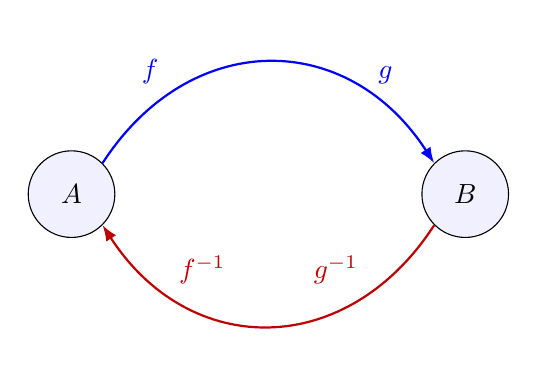
\begin{tikzpicture}[
  auto,
  object/.style={draw,circle,minimum size=11mm,fill=blue!6},
  morphism/.style={-{Latex[length=2mm]},thick}
]
  \node[object] (A) at (0,0) {$A$};
  \node[object] (B) at (5,0) {$B$};

  \draw[morphism,blue] (A.north east) .. controls (1.5,2.1) and (3.5,2.1) .. (B.north west)
    node[pos=.22] {$f$}
    node[pos=.78] {$g$};
  \draw[morphism,red!75!black] (B.south west) .. controls (3.5,-2.1) and (1.5,-2.1) .. (A.south east)
    node[pos=.22,swap] {$g^{-1}$}
    node[pos=.78,swap] {$f^{-1}$};
\end{tikzpicture}
\end{document}
